\section{Introduction}

Decision-making under partial observability requires agents to balance exploiting current knowledge against gathering information to reduce uncertainty about hidden states. In a standard partially observable Markov decision process (POMDP), information gathering has no intrinsic value. It is useful only insofar as it leads to higher expected reward. This creates a well-known difficulty. A reward-only planner values an observation only if it looks far enough ahead to see the reward that the observation eventually buys. The exploration--exploitation trade-off must therefore be resolved either by a planning horizon deep enough to see that far or by heuristic exploration bonuses.

The $\rho$-POMDP framework \citep{araya2010} addresses this by extending POMDPs with a belief-dependent utility $\rho(b)$ that allows the agent to derive value directly from properties of its belief state. This enables explicit optimization over uncertainty reduction, information gain, or other belief-state properties alongside task reward. However, the choice of $\rho$ remains largely heuristic and environment-specific, and, when $\rho$ is an information-gain term, so does the weight placed on it.

This paper treats that weight as a design problem with a resource-allocation answer. Most of the environments we study pose an observe-then-commit (OTC) problem. Each observation costs something, and the agent gathers as many observations as it chooses before committing to a terminal decision whose payoff depends on the hidden state. In that setting a natural design input is a sensing budget $B$, the amount of sensing the agent is expected to use before committing, stated as an expectation over episodes rather than as a hard per-episode limit. A target of that kind arises when sensing is itself a deliverable, as in a coverage, monitoring, or verification requirement that fixes how many inspections are to be made regardless of what the task reward alone would justify, and the question is then which weight delivers that expected usage. We measure that amount as sensing usage, the expected number of observation actions (tests, scans, or checks) the agent takes per episode, and $B$ is stated in the same units (Section~\ref{sec:budget_theory}). The budget sections also allow usage to be denominated in cumulative sensing cost instead, but throughout this Introduction usage means the count. The proposal is to state that budget and to price the information-gain utility at the budget's \emph{operational shadow price} $w^*(B)$, the weight at which the agent's expected usage crosses $B$. Where the usage curve jumps over $B$, so that no single weight meets it exactly, the price is still that one crossing weight, and the procedure estimates it by a bracket of neighboring grid weights, as the next paragraph explains. In constrained optimization, a shadow price is the marginal value of one more unit of a scarce resource, obtained as the Lagrange multiplier on that resource's constraint, and the adjective operational marks a deliberate departure from that meaning. Our price is read off a usage curve, the map from weight to the agent's expected usage, rather than obtained as that multiplier, and Section~\ref{sec:budget} makes precise what $w$ is and is not a multiplier of. The question ``what weight should the information-gain utility carry'' becomes ``what expected sensing usage do we intend,'' with the weight read off the stated usage target rather than searched per task.

Four properties make this price useful in practice. It can be estimated offline, tracked online, and rescaled with rewards. When the usage curve jumps over a budget, a crossing bracket estimates the price and an endpoint mixture can attain the budget in expectation. Offline, the price is computable from that usage curve (Section~\ref{sec:budget}). Online, it is trackable by dual descent, a feedback rule that nudges the weight down whenever measured sensing usage runs above the target and up whenever it runs below it. For the projected, decaying-step form of that rule, stationary convergence is guaranteed under stated conditions (Proposition~\ref{prop:pi5}), and re-adaptation under mid-run reward-scale shift is demonstrated empirically (Section~\ref{sec:dual_multiseed}). Under rescaling, the price is scale equivariant for the receding-horizon planner the paper implements, one that re-plans from its current belief at every step and executes only the first action of each plan, exactly in the mathematics and up to floating-point rounding in code. Equivariance here means that multiplying every reward and cost by a constant $\alpha>0$ multiplies the price by the same constant, so that the count-usage curve at the new scale is the unscaled curve read against $w/\alpha$ in place of $w$, while a cost-usage curve also rescales by $\alpha$. The price at a rescaled problem is therefore obtained by multiplying the old price by $\alpha$, not by searching for it again (Proposition~\ref{prop:pi1}). The fourth property follows from the shape of the usage curve. The agent chooses each action by comparing finitely many alternatives, so a small change in $w$ either leaves its policy, and with it its sensing usage, unchanged or switches it. A switch can move usage by a whole observation at once. The usage curve is therefore a staircase. It is not always monotone, because a switch at a higher weight can, for example, trade several weak observations for fewer but individually more informative ones (Section~\ref{sec:pi2} gives the full account). No single weight exactly meets a budget inside a staircase jump. At such a usage gap the crossing threshold is still a single number, the location of the jump, and the procedure reports it as a crossing bracket, the pair of neighboring grid weights that straddle the jump, together with a per-episode mixture of the two endpoint policies that attains the budget in expectation (Definition~\ref{def:pi3}). The bracket's width is grid resolution, not an interval of exact prices.

The active inference (AIF) framework \citep{friston2010, parr2019} identifies one canonical point on this price curve. AIF casts perception and action as approximate Bayesian inference, selecting policies that minimize Expected Free Energy (EFE). EFE naturally decomposes into a pragmatic term (goal-seeking) and an epistemic term (information-seeking). Because both terms come from a single variational objective, their relative coefficient is fixed once pragmatic value is identified with task reward. In the discrete-state formulation we use, that coefficient is $w{=}1$ in information units, one reward unit per unit of information (Proposition~\ref{prop:equivalence}). The claim is exact under log scoring rules \citep{bernardo1979}, rewards that pay the agent the log probability it assigned to the outcome that occurred, so that reward is already measured in information units. Under a shared reward convention, a fixed exchange rate between the units of task reward and the information units of the epistemic term, it is an empirically robust untuned default. That default is not scale-invariant. Multiplying every reward and cost by $\alpha>0$ leaves the bit-valued information term unchanged, so a fixed $w{=}1$ implements a different trade-off at every scale. Rather than treating this as a limitation to caveat, we read it as confirmation that $w$ is a price. In the budgeted formulation above, $w{=}1$ is then one of the weights whose expected usage equals the budget it happens to imply at the ambient reward scale, not a universal, scale-invariant calibration. A convention-free comparison between a reward-denominated quantity and a bit-denominated one is not on offer to any fixed weight, ours included. The log-scoring derivation gives a principled anchor within this unavoidable choice of units, while leaving the reward convention itself to the designer.

Figure~\ref{fig:hero} shows how a sensing target is read from the price curve. Figure~\ref{fig:engineering_workflow} places that calculation in an engineer's inspection workflow.

\begin{figure}[!t]
\centering
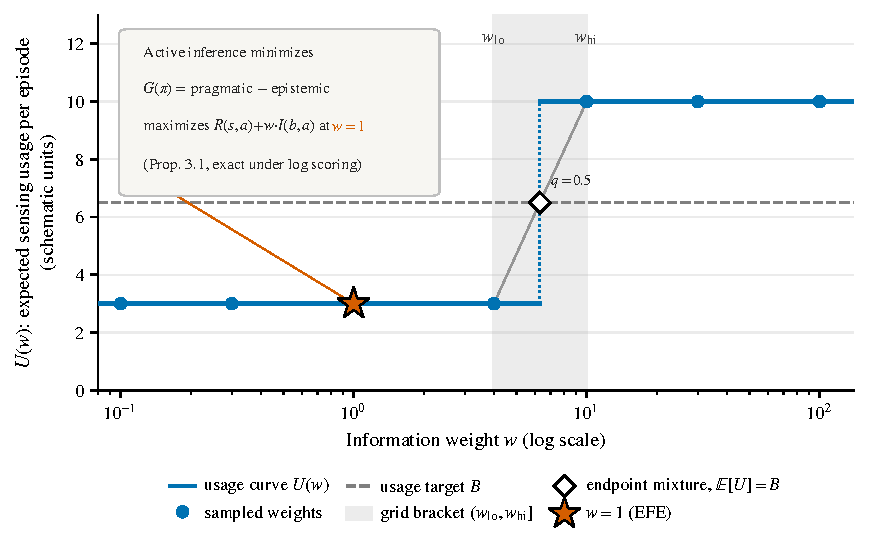
\includegraphics[width=\linewidth]{figures/fig_hero_price_curve_jair.pdf}
\caption{A schematic price curve for an information-gain weight (illustrative, not measured data). The blue curve is a usage curve $U(w)$, the expected sensing an agent uses at information-gain weight $w$, drawn with one jump between two sampled grid weights (dots). Measured usage curves elsewhere in this paper carry further plateaus, jumps, and occasional dips and are not asserted to be monotone. A stated expected sensing budget $B$ (dashed line) is a target for expected usage, not a per-episode cap. Here it falls inside the usage gap the jump opens, so no single weight attains it and the level set of Definition~\ref{def:pi3} is empty. The dotted riser at an unsampled weight is the crossing threshold, and the shaded band is the crossing bracket $(w_{\mathrm{lo}}, w_{\mathrm{hi}}]$, the grid's estimate of where that threshold lies, a grid interval rather than a set of prices. The open diamond on the budget line is the endpoint mixture, a randomized policy that plays $w_{\mathrm{hi}}$ with probability $q$ and $w_{\mathrm{lo}}$ otherwise, drawn afresh each episode, and so attains $B$ in expectation (here $q{=}0.5$), with leader lines to the two grid points it mixes. The boxed aside states the equivalence result in the notation of the axes. Minimizing the recursive, reward-based Expected Free Energy objective we specify is exactly equivalent to maximizing $R(s,a) + w \cdot I(b,a)$ at $w{=}1$ for observe-then-commit POMDPs and for the hidden-state-preserving actions of factored observation POMDPs, exact under log scoring rules (Propositions~\ref{prop:equivalence} and~\ref{prop:factored}). The star marks that $w{=}1$ on the curve, derived from the objective rather than tuned, and sitting outside this particular bracket. The price is scale equivariant for the receding-horizon planner (Proposition~\ref{prop:pi1}), so rescaling every reward and cost by a constant rescales $w$ by the same constant and leaves this count-usage curve unchanged once it is read against the rescaled weight, and $w{=}1$ is one weight whose expected usage equals the budget the ambient reward scale happens to imply, not a universal number.}
\label{fig:hero}
\Description{A single line chart on a light background, with no photographic content. The horizontal axis is labeled information weight w and uses a log scale running from about 0.1 to 100. The vertical axis is labeled U of w, the expected sensing usage per episode in schematic units, running from 0 to about 13. A blue line stays flat at a low value of 3 from the left edge to a weight of about 6, jumps vertically there along a thin dotted blue riser to a high value of 10, and stays flat at 10 to the right edge. Seven blue dots mark the sampled grid weights at 0.1, 0.3, 1, 4, 10, 30, and 100, the first four on the low plateau and the last three on the high plateau. This single jump is drawn as a clean illustrative simplification, not as measured data, and usage curves reported elsewhere in this paper can include additional plateaus, jumps, or small non-monotone dips. A horizontal gray dashed line crosses the full width of the plot at a height of 6.5, between the two plateaus, representing a stated expected sensing budget B that no single sampled weight attains. A light gray vertical shaded band spans from the grid weight 4 up to and including the grid weight 10, labeled w-low and w-high near its top left and top right corners, marking the crossing bracket, the grid's estimate of where the curve crosses the budget. Where the dashed budget line meets the dotted riser, an open white diamond with a black outline marks the endpoint mixture, the randomized policy that plays w-high with probability q and w-low otherwise, and a small label beside it reads q equals 0.5. Two thin gray leader lines connect the diamond to the grid point at weight 4 on the low plateau and the grid point at weight 10 on the high plateau, the two endpoints it mixes. A black-outlined vermillion five-pointed star sits on the curve's low plateau at w equals 1, positioned clearly to the left of and outside the shaded band. A thin vermillion line connects the star to a small rounded text box in the upper left of the plot, an area with no curve or other data in it. The text box's right edge stops with a clear gap of open space before the shaded band's left edge. The text box states, on four lines, that minimizing Expected Free Energy, written as G of pi equals a pragmatic term minus an epistemic term, is exactly equivalent to maximizing a rho-POMDP objective, reward of s and a plus w times information gain of b and a, at w equals 1, and that this identity is exact under log scoring rules, citing the equivalence proposition by number. Within that box, only the text w equals 1 is printed in the same vermillion color as the star, and every other word in the box is plain dark text. A frameless legend in three columns below the plot lists six items, the blue curve, the sampled grid weights, the dashed budget line labeled as a target, the shaded crossing bracket labeled as a grid estimate, the endpoint mixture diamond with its expected usage equal to B, and the star. Read together, the figure shows expected sensing usage jumping with an information-gain weight, a stated budget falling in the gap so that the sampled grid can only bracket the crossing, a separate randomized mixture of the two bracket endpoints attaining the budget in expectation, and a single labeled point on the same curve, the weight that active inference derives on its own, shown as forced by a theorem rather than chosen by hand, and shown sitting outside the particular bracket drawn here rather than coinciding with it.}
\end{figure}

\begin{figure}[!t]
\centering
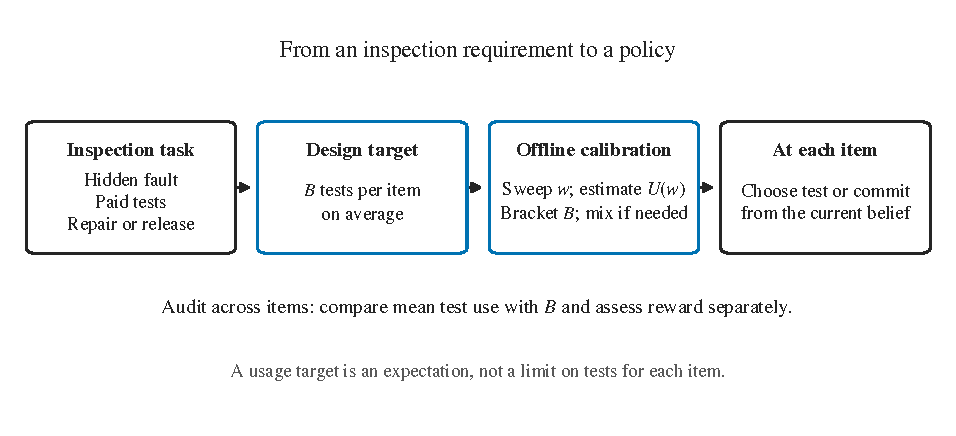
\includegraphics[width=\linewidth]{figures/fig_engineering_workflow.pdf}
\caption{From an inspection requirement to a running policy (schematic, not experimental data). For a state-preserving task with a hidden fault and paid tests, the engineer states a target $B$ in expected tests per item. An offline sweep estimates usage $U(w)$ and brackets $B$; when a usage gap lies between the selected endpoint policies, mixing them across items can meet the target under Definition~\ref{def:pi3}'s conditions. The deployed agent chooses tests and terminal actions from its current belief. Usage and reward are assessed separately: meeting $B$ does not establish reward optimality under a sensing cap.}
\label{fig:engineering_workflow}
\Description{A four-stage horizontal flow chart headed From an inspection requirement to a policy. The boxes read: Inspection task, hidden fault, paid tests, repair or release; Design target, B tests per item on average; Offline calibration, sweep information weight w, estimate usage U of w, bracket B and mix if needed; At each item, choose test or commit from the current belief. Arrows connect the boxes left to right. Below them a line says to audit mean test use against B and assess reward separately. A final line says the usage target is an expectation rather than a limit on tests for each item.}
\end{figure}

The two figures answer different practical questions. Figure~\ref{fig:hero} shows which weight a specified usage target selects, including what to do when the usage curve jumps over it. Figure~\ref{fig:engineering_workflow} shows what an engineer must supply and check: a model of tests and outcomes, an expected-usage target when that is the design requirement, calibration runs to estimate the usage curve, and a separate assessment of reward. The agent still chooses each observation or commitment from its updated belief; the budget selects the policy family member rather than prescribing a fixed number of tests for every item.

Our contributions are as follows.\footnote{Code and experiment data are available at \url{https://github.com/PatrickAllenCooper/rho_aif}.}
\begin{enumerate}
    \item Budgeted reformulation. We recast the information weight as the operational shadow price $w^*(B)$ of a sensing budget $B$ (Section~\ref{sec:budget}), prove exact scale equivariance of the resulting policy family for the receding-horizon planner under the scale-independent tie-break the implementation uses (Proposition~\ref{prop:pi1}), separate the level set, the crossing threshold, the finite-grid crossing bracket, and the endpoint mixture at usage gaps (Definition~\ref{def:pi3}), and give an online dual controller, a projected decaying-step recursion, with a stationary convergence guarantee under stated conditions (Proposition~\ref{prop:pi5}). In experiments, that controller, whose step size shrinks over time, re-adapts after a mid-run reward-scale shift. With an added change-detection heuristic that restarts the step-size schedule when it declares a shift, it re-adapts on all ten controller seeds tested, and without that heuristic on nine of the ten inside the post-shift window, roughly three times more slowly on a recovery-time estimand defined for every seed (Section~\ref{sec:dual_multiseed}). This is the paper's primary contribution. It turns a hyperparameter into the price of a stated expected sensing usage target.
    \item Theory. A formal bridge between $\rho$-POMDPs and active inference, which is what licenses reading $w{=}1$ as an anchor on the price curve rather than an arbitrary choice. We prove the equivalence for observe-then-commit POMDPs (Proposition~\ref{prop:equivalence}), characterize when the information-unit weight $w{=}1$ is near-optimal (Proposition~\ref{prop:nearopt}), and extend the equivalence to factored observation POMDPs (Proposition~\ref{prop:factored}). A factored observation POMDP (Definition~\ref{def:factored}) splits the state into a fully observable part and a hidden part. Its actions come in three kinds, namely observation actions that look at the hidden part, navigation actions that move the agent without touching the hidden part, and exploitation actions that collect reward that depends on the hidden part. Observing and moving may interleave with exploiting rather than precede a single commit, and the extension covers the case in which the observation and navigation actions preserve the hidden state.
    \item Evidence. The empirical evidence comes in two batteries, one for each theoretical contribution. The first exercises the budgeted formulation of Contribution~1, and the second evaluates the equivalence results of Contribution~2. The second battery runs controlled comparisons across five OTC environments, namely Tiger, Diagnosis, Bandit, Tileworld, and the two-state Testbed, and the first battery adds a sixth, the distractor variant of Diagnosis (Section~\ref{sec:distractor}). Navigation, a further environment whose study is reported in Appendix~\ref{app:navigation}, is counted separately because it has only move actions, with no observation actions and no terminal commit, so it falls outside the OTC class as defined above. The two principal baselines are same-horizon planning (hereafter Planning), a reward-only planner that looks ahead to the same depth as the EFE agent, and tuned information gain (Planning+IG), the same planner with a tuned information-gain bonus added to its objective. POMCP \citep{silver2010}, an online Monte Carlo tree-search planner for POMDPs, is a further baseline on the first four of those environments. The suite also includes four instances of a cost-modified RockSample variant \citep{smith2004}. Section~\ref{sec:experiments} states the six deviations from the original benchmark, and Appendix~\ref{app:rocksample} reports a full tree-search POMCP with a tuned, frozen configuration on all four instances, distinguished there from a flat one-ply Monte Carlo reference. A Pareto analysis, which sweeps $w$ and places each weight on a success-rate versus reward frontier, shows that on Diagnosis and Bandit, $w{=}1$ Pareto-dominates Planning, reaching higher success with comparable or better reward, while remaining competitive with tuned Planning+IG across environments. The first battery (Section~\ref{sec:budget_experiments}) exercises the budgeted formulation in five ways. It shows usage-curve collapse across reward scales, meaning that curves measured at different reward scales coincide once the weight is rescaled with them. It shows the closed-form onset thresholds, the weights at which sensing first turns on, recovered as the first jump of the measured usage staircase. It shows the online dual controller tracking a stated budget, across seeds, through a $\times 10$ reward rescale. It tests the calibration procedure at target budgets set by a predeclared rule from the calibration curve's range, independent of the weight-one usage though not application-specified, on held-out seeds, and reports where meeting a budget earns reward and where it costs reward relative to the best budget-feasible single weight and to a near-optimal constrained reference. And it shows a near-optimal reference computed by SARSOP, an offline point-based POMDP solver, statistically equivalent to EFE ($w{=}1$) on the three core OTC environments (Tiger, Diagnosis, and Bandit) by the two one-sided tests (TOST) procedure at a fixed sensing-cost margin, an equivalence test that supports, rather than merely fails to reject, the conclusion that the two agents differ by less than the stated margin.
    \item Practical guidance. We identify the tested conditions under which EFE-as-$\rho$ helps and the model structures in which information gain fails by construction. In the tested regimes, the advantage appears when the agent must choose among multiple observation actions. We isolate that dependence directly on the Diagnosis task, in which the agent must identify one of $N$ hidden conditions using $K$ available tests, by holding the environment fixed and varying only the number of tests (Appendix~\ref{app:obs_scaling}). There, at $N{=}8$, the success-rate gap between EFE and reward-only planning is zero at $K{=}1$, within sampling error at $K{=}2$, and $+13.2$pp (percentage points) at $K{=}3$. The main battery's Diagnosis instance, which has two tests at a smaller $N$, supplies the corresponding $K{=}2$ evidence in Table~\ref{tab:main}.

    The advantage also opens at the largest scale of the Tileworld sweep ($69.4\% \pm 1.0$pp vs.\ $1.4\% \pm 0.3$pp success, seed-level SE, at $8{\times}8$, Section~\ref{sec:results}). Tileworld's observation actions are scans, each a noisy yes/no question about the location of a hidden target tile. At that grid size and the sweep's fixed lookahead depth, no scan repays its cost before the lookahead ends and the planner must value a commit. Reward-only Planning therefore stops scanning entirely, while EFE, searching to the same depth but crediting each scan's expected information gain directly, does scan. The comparison there is therefore EFE against a non-scanning agent, a joint horizon-and-scale effect rather than a pure scale effect. That result invites the reading that the advantage grows with problem size, a reading the abridged workshop version of this article made and that we revise below. What our results actually support is narrower than a size law. The advantage tracks how much slack a problem's structure leaves between what the reward-only planner does on its own and the information-optimal behavior that the agent's search can actually represent. On Tileworld that slack is the room between never scanning and the scanning that the same depth-limited search can represent, and it correlates with size there but not in general.

    RockSample makes the point. In the bracket notation RockSample[$\cdot$,$\cdot$], the first entry is the side of the square grid and the second is the number of rocks whose hidden quality the agent may check. The second entry therefore counts the observation actions and plays the role of the $K$ of the Diagnosis sweep. On RockSample, the advantage is largest with several rocks to check ($+9.54$ reward over reward-only Planning on RockSample[7,8], $K{=}8$) but does not persist to every instance we test, vanishing on RockSample[11,11] ($K{=}11$) where every tree-search agent scores within sampling error of every other. On the two larger instances a hand-coded unbounded-horizon heuristic beats all of them, which bounds what these instances can be asked to show about weighting and locates the limitation in the depth of the search rather than in the epistemic term (Section~\ref{sec:rocksample}).

    Two structural limits accompany these results. Ordinary information gain is reward-blind, so it will spend a sensing budget reducing uncertainty that has no bearing on reward. A variant that weights information by its relevance to reward eliminates that wasted spending entirely at every weight in the sweep, and it does so using only quantities the agent already holds (Section~\ref{sec:distractor}). Naive information gain can also misvalue an action outright when observing changes the hidden state (Example~\ref{ex:destructive}).
\end{enumerate}

An abridged version of this article was accepted as a poster and spotlight presentation at the 7th International Workshop on Active Inference (IWAI 2026) \citep{cooper2026iwai}. It comprised the equivalence results in Contribution~2 above (Propositions~\ref{prop:equivalence}, \ref{prop:nearopt}, and \ref{prop:factored}) and the second experiment battery of Contribution~3. This article is a substantially extended version. The entire budgeted $\rho$-POMDP formulation of Section~\ref{sec:budget} (Definition~\ref{def:pi3} and Propositions~\ref{prop:pi1}, \ref{prop:pi2}, \ref{prop:pi5}, and Corollary~\ref{cor:pi4}), the first experiment battery of Section~\ref{sec:budget_experiments}, and the distractor and destructive-sensing results of Contribution~4 are new material that was not part of the IWAI submission. Contribution~4 otherwise revises the IWAI version's characterization, which claimed the advantage grows with state space size and observation action count, a claim RockSample[11,11] does not support.

The remainder of the article is organized as follows. Section~\ref{sec:methodology} sets up OTC $\rho$-POMDPs and EFE, states the equivalence and near-optimality results of Contribution~2 with proof sketches (the full proof of Proposition~\ref{prop:equivalence} is in Appendix~\ref{app:proof}), and introduces the agent family used throughout. Section~\ref{sec:budget} develops the budgeted formulation of Contribution~1, including the crossing bracket and endpoint mixture, the scale-equivariance result, and the online dual controller. Section~\ref{sec:experiments} describes the environments and the statistical protocol. Section~\ref{sec:budget_experiments} reports the first experiment battery, which evaluates the budgeted formulation, and Section~\ref{sec:results} reports the second, which evaluates the equivalence results. Section~\ref{sec:discussion} takes up scope and limitations before the conclusion. We first situate the work in the related literature.
